% Put the project details here

\section{PROJECT DETAILS}

        \subsection{Overview}
        Chirin Ivatan is a web-based Community-Based Information System (CBIS) designed to document, preserve, and promote the Ivatan language and folklore. This chapter presents an overview of the proposed system. Designed especially for the Ivatan community and future generations, Chirin Ivatan will be built using mostly free, open-source tools to ensure that it remains affordable and sustainable. This chapter outlines the overall structure of the project, the technologies to be used, the system’s design, and the step-by-step plan for building and implementing it. By integrating modern technology, the system ensures the preservation of linguistic and cultural heritage while engaging younger generations through gamified learning experiences and community contributions.
        \subsection{Project Framework}
        The project framework provides a structured approach to align the project’s objectives with its implementation, ensuring that all aspects—from system design to user engagement—are coherently developed and systematically managed. 

        At its core, the Chirin Ivatan project follows a user-centered design approach. This means that the system is being developed with a strong focus on the people who will actually use it—especially the Ivatan community. From the early planning stages through to the final product, the preferences, needs, and feedback of users will help guide the design and features of the platform. This is important because the project is not just about creating a website; it's about building a meaningful and useful platform for the Ivatan people and researchers. 

        To make this process organized and flexible, the project will use the Agile Software Development method. Agile is a way of managing projects that focuses on building the system step by step instead of trying to complete everything all at once. The work is divided into shorter time periods focusing on one part of the system at a time—such as the dictionary module, audio features, or folklore archive. After each part, the progress will be tested for feedback. Agile is a good fit for this project because it allows for adjustments along the way, which is especially helpful since development is expected to be slower and because community input is a key part of the system’s success.

        The framework is composed of the following key components:
            \subsubsection{Project Objectives and Design}
            The main goal of Chirin Ivatan is to create an easy-to-use, sustainable digital platform that preserves and promotes the Ivatan language and folklore. The project will focus on building four main features:an Ivatan-English dictionary with audio pronunciation, a section for documenting folklore such as stories, proverbs, and songs, user accounts that allow people to contribute and review content, and interactive learning tools like quizzes and leaderboards.

            This stage also includes identifying user needs, designing how the system will work, and making sure the layout and interface are friendly and accessible for all users, especially those with limited tech experience or internet access.
            \subsubsection{Development Phase and Technology Strategy}
            The development will begin with building the basic features using beginner-friendly and cost-effective tools. At first, the backend will use Firebase for user login, database storage, and hosting, while the frontend will use React.js to build the interface. These tools are ideal for fast testing and building simple versions of the platform. The platform will switch to using Django (Python) and PostgreSQL for better data handling and more advanced features. The Web Audio API will be used to play pronunciation recordings directly on the platform.
            \subsubsection{Testing and Refinement}
            After building each part of the system, tests will be done to check if everything works well and is easy to use. Feedback will be gathered from a few tentative users, especially Ivatan community members, to help improve the system before moving forward.
            \subsubsection{Deployment and Community Participation}
            Once the platform is ready, it will be launched and shared with local institutions, schools, and cultural groups in Batanes. A big part of this project is community involvement. Native Ivatan speakers, teachers, and culture bearers will be encouraged to add entries, check the accuracy of content, and suggest improvements. Surveys, feedback sessions, and consultations will be done regularly to make sure the platform truly reflects the community’s language and stories. The following are tentative agencys bthat are planned to be presented to and asked for feedback:
                \begin{itemize}
                \item The Department of Education Division Office of Batanes through the Education Program Supervisor incharge of Indigenous People Education, Mr. Jay V. Gonzales
                \item The Batanes State College
                \item The Batanes Heritage Foundation Inc. through its current President Ms. Catherine de Mata
                \item The Provincial Tourism Office of Batanes through the Provincial Tourism Officer Ms. Hegel B. Valones
            \end{itemize}
            \subsubsection{Knowledge Management and Documentation}
            All steps of the project—from building the platform to uploading content—will be carefully documented using GitHub, this manuscript, system documentation, and a user guide. Special attention will be given to ethical archiving practices to protect and respect Ivatan cultural heritage, especially when handling oral traditions, stories, and community-contributed content.
            By openly sharing the project’s methods, challenges, and solutions, Chirin Ivatan aims to become a valuable benchmark for other indigenous communities and digital heritage projects. The framework can be adapted by similar initiatives looking to preserve their own languages and traditions using accessible technologies and community-driven strategies. In this way, Chirin Ivatan is not only a local tool for preservation, but also a model that can inspire and guide others working toward cultural sustainability in the digital age.
            \subsubsection{Evaluation and Sustainability Planning}
            The project will track its progress through measurable indicators like the number of registered users, contributions made, and how often the platform is used. Feedback will be collected often to guide improvements. To ensure the project lasts beyond the initial development, possible partnerships or even turnover will be explored with NGOs that support indigenous heritage. More than it is feature driven, the main goal is to keep the platform active and reliable for as long as possible so keeping it well documented and low maintenance is key. \\
            
            The Chirin Ivatan project framework provides an adaptive structure that integrates community involvement, iterative development, and cultural sensitivity. It ensures that the platform is not only a technological product but also a living, evolving initiative rooted in service to the Ivatan people.


            
        \subsection{Materials/Technologies Used}
        The following selection of technologies for Chirin Ivatan is grounded in accessibility, scalability, and open-source availability. The goal is to use free or low-cost tools where possible while still laying the foundation for a long-term sustainable platform. The approach also supports a progressive learning path, wherein the proponent gains familiarity with the full-stack development tools needed for the system’s actual implementation.

                \begin{itemize}
                \item Frontend Framework- Basic web technologies such as HTML, CSS, and JavaScript will be used initially to build static pages and interactive elements. React.js may be incorporated to create a more responsive and engaging user experience, particularly for the gamified learning components of the system.
                \item Cloud Platform (for prototyping)- Firebase will be used during the prototyping phase due to its integrated services such as user authentication, real-time database, and hosting—all available under a free tier. Firebase allows for quick deployment and testing of MVP features. It will later be replaced by a more scalable Django-based backend once development continues.
                \item Programming Language- Python is chosen as the main programming language for backend development due to its readability, and versatility. It is also widely used in academic and professional settings, making it an ideal starting point for the proponent. Python will serve as the language for server-side logic, data processing, and integration of backend components.
                \item Web Framework- Django will be used to structure the backend of the platform. Django promotes development and clean, pragmatic design, which is ideal for a solo developer with limited prior experience. It also includes built-in features such as user authentication, admin interface, and Object-Relational Mapping, reducing the need for manually coding common web development components. This will allow the developer to focus more on building core functionalities such as the dictionary module, folklore database, and content contribution system.
                \item Database System- During the early stages of development, Django’s default SQLite database will be used for ease of local testing. For production deployment and scalability, the system will be upgraded to PostgreSQL. PostgreSQL will be essential for handling more complex queries, user contributions, and metadata associated with folklore entries and audio files.
                \item Audio Integration- To support pronunciation guides and oral storytelling components, the project will make use of the Web Audio API for integrating native audio playback. This allow users to listen to word pronunciations and folklore recordings without needing any additional plugins, making it ideal for a community like the Ivatans where most are still new to using gadgets. 
                \item Version Control- Version control will be managed using Git hosted on GitHub. This ensures proper documentation, tracking of changes, and future collaboration opportunities with fellow developers or community contributors. 
                \item Hosting and Domain Services (To Be Determined)- Development will initially occur in a local environment or through Firebase’s free hosting but deployment for public access will require hosting and domain services. Hosting and domain will likely be the only paid components of the system, as all other technologies are free or open-source.
            \end{itemize}
        The development of Chirin Ivatan will strategically utilize free and beginner-friendly technologies while progressively integrating more advanced tools as the proponent’s technical capacity improves. This approach ensures that the platform can be developed sustainably while meeting the project’s objective and the community needs.


        
        \subsection{System Design}
        The following outlines both the functional and non-functional requirements of the platform, as well as the proposed architecture, user interactions, and database schema. As a community-based information system, the design emphasizes simplicity, scalability, and user-friendliness to serve both native Ivatan contributors and general users seeking to explore the language.
        \subsubsection{Functional Requirements}
        These are the core features and capabilities that the system must perform to meet user needs:
            \begin{itemize}
                \item User Registration and Authentication- Users must be able to register, log in, and log out securely. There will be roles such as general user, contributor, and administrator.
                \item Dictionary Module- Users can search for Ivatan terms and view their definitions, English translations, example sentences, and audio pronunciation.
                \item Programming Language- Python is chosen as the main programming language for backend development due to its readability, and versatility. It is also widely used in academic and professional settings, making it an ideal starting point for the proponent. Python will serve as the language for server-side logic, data processing, and integration of backend components.
                \item Folklore Module- Allows browsing and submission of Ivatan stories, legends, proverbs, and oral traditions. Admins can moderate submitted content.
                \item Content Contribution System- Authenticated contributors can submit new dictionary entries or folklore items, subject to admin review and approval.
                \item Gamified Learning Tools (Planned Feature)- Includes quizzes and leaderboards to make language learning interactive and engaging, especially for younger users.
                \item Mobile-Friendly Interface- The platform must be accessible and readable on mobile devices and desktops with varying screen sizes and connection speeds.
            \end{itemize}
        \subsubsection{Non-Functional Requirements}
        These define how the system should perform:
            \begin{itemize}
                \item Scalability- The system should be able to handle more users and content as the platform grows. It will start with Firebase for fast prototyping and ease of use, then move to Django with PostgreSQL later on to support a larger database and more advanced features.
                \item Maintainability- The codebase should be organized and so that updates, bug fixes, or changes can be made easily. Clear comments and consistent naming conventions will be useful to keep this.
                \item Performance- The platform should load and respond to user actions (like searching or clicking through pages) within 2–5 seconds- which is ambitious but possible because of connectivity challenges in the islands of Batanes where most users reside. Lightweight design and optimized queries will be used to achieve this.
                \item Security- Basic security features will be implemented to protect user data and the integrity of the content. These include password hashing, role-based access control and proper input validation to avoid common vulnerabilities.
                \item Accessibility- The platform will be simple to use and designed with users in mind who may not be tech-savvy or have strong internet connections. It will work well on mobile devices and offer intuitive simple navigation.
                \item Cost-Efficiency- To keep the project affordable, most tools and services used will be free or open-source. Paid services will be limited to essentials like hosting, a domain name, or others when needed. This makes the system sustainable even with limited funding.
            \end{itemize}
        
        \subsection{Implementation}
        The implementation follows a structured, phased approach that considers both the academic schedule of the IS295 course sequence and the proponents current capacity. The months before full system development will focus on skill-building, early content gathering, and community engagement. Full development, testing, and deployment are scheduled between January and April 2026, during IS295B to allow enough time for testing of user-contributed content and system features.
                \subsubsection{Pre-Implementation (Preparation and Capacity Building) Phase}
                This six-month phase is focused on preparation, learning, planning, and gathering of initial content. This will also allow time for the proponent to gain the needed skills for implementation. The main goals are to build foundational technical skills, outline system features, and begin early engagement with users and content contributors.
                \begin{itemize}
                \item Design and User Flow Planning (July 2025)- Wireframes and simple user flows will be created using Figma. This will help visualize how users navigate through the platform and interact with features.
                \item Prototype and Feature Planning (August – October 2025)- A basic prototype will be developed using Firebase or simple static HTML templates. This phase focuses on experimenting with layouts, testing basic features and finalizing core modules and data structures.
                \item Initial Content Collection (October 2025)- The proponent will begin collecting Ivatan vocabulary and folklore materials like myths and proverbs from existing sources and personal outreach. This will form the initial content for the platform—populated before user submissions begin.
                \item User Research and Early Collaboration (October 2025)- Consulations with the listed agency’s and with potential users such as Ivatan educators, students, and cultural advocates will be conducted. Their feedback will inform design decisions and help ensure the system is culturally respectful and easy to use.
            \end{itemize}  
                \subsubsection{Development and Implementation Phase }
                This phase marks the formal development and rollout of the Chirin Ivatan platform during IS295B.
                \begin{itemize}
                \item Backend Development (January  – February 2026)- Using Django backend features such as user registration, content submission, moderation tools, and dictionary management will be built.
                \item Frontend Development (January– February 2026)- The user interface will be developed using HTML, CSS, and JavaScript. Interactive parts (like the games or quizzes) will be enhanced using React.js.
                \item Database Integration (January– February 2026)- Development will begin with SQLite for testing, then migrate to PostgreSQL.
                \item Audio Playback Features (January 2025 – February 2026)- Audio recordings for pronunciation and storytelling will be integrated using the Web Audio API. The system will support uploading and playback of audio clips for dictionary and folklore entries.
                \item Testing and Debugging (January – February 2026)- Each system module will undergo functionality and usability testing. This will be used to identify bugs and make improvements before launch.
                \item Deployment (February 2026)- The final system will be deployed using a budget-friendly hosting service. Costs will be limited to essentials like hosting and a domain name. This phase also marks the start of data collection from real users contributing to the knowledge base.
            \end{itemize} 

    \textit{This section will be completed with actual results and screenshots during IS295B after the final system is built and tested.}\\\\
    The following are gantt charts for each of the 2 major stages: 

    \begin{figure}[ht]
    \begin{center}
        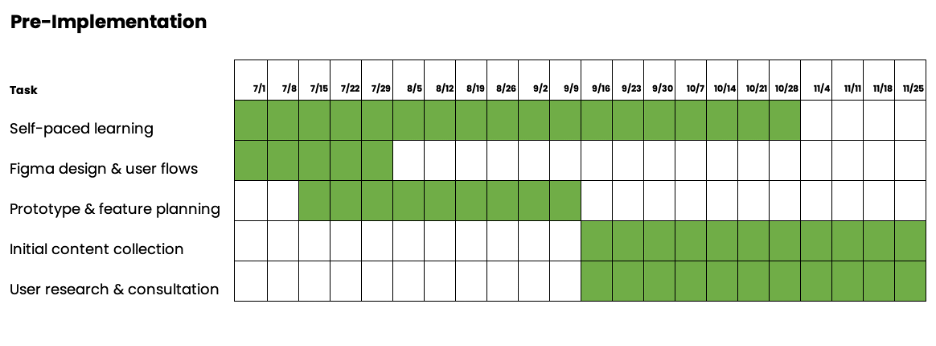
\includegraphics[width=480px]{Texfiles/images/preimp.png}
    \end{center}
        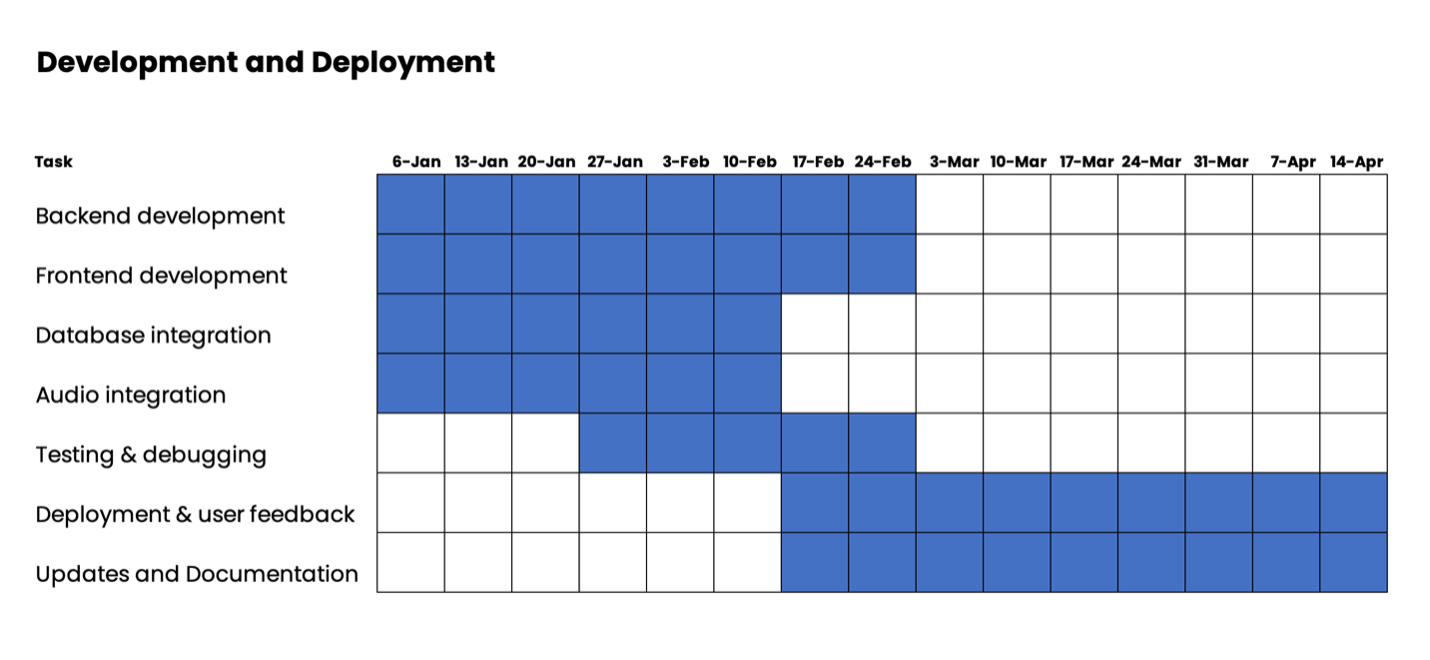
\includegraphics[width=480px]{Texfiles/images/devt.png}
    \end{figure}